%%%%%%%%%%%%%%%%%%%%%%%%%%%%%%%%%%%%%%%%%%%%%%%%%%%%%%%%%%%%%%%%%
%        Contents: Bachelorarbeit, HS Fulda        %
%                          06.09.2022                        %
%---------------------------------------------------------%
%                            Konzept.tex                     %
%                         by Fangfang Tan                    %
%         fangfang.tan@informatik.hs-fulda.de      %
%%%%%%%%%%%%%%%%%%%%%%%%%%%%%%%%%%%%%%%%%%%%%%%%%%%%%%%%%%%%%%%%%

\chapter{Untersuchung weiteren Funktionen} \label{UF}

In Kapitel 3 wurden Funktionen beschrieben, die im Rahmen dieser Arbeit technisch umgesetzt wurden. Dieses Kapitel betrachtet weitere Standard-Anforderungen  an Webanwendungen im SAP-Kontext und Funktionaltitäten von Fiori Elements, SAP AppGyver und SAPUI5, ohne praktische Umsetzung. Diese Funktionen umfassen: 

\begin{itemize}[noitemsep]
\item Integration von Suchfiltern und Paginierung. 
\item Integration von Bildern und PDF-Dateien.
\item Integration einer Barcode-Scanner-Funktionen.
\item Nutzung weiterer mobiler Funktionen. 
\item Möglichkeiten zum Deployment für unterschiedliche Endgeräte
\item Freie Gestaltungsmöglichkeiten in der UI
\end{itemize}

\section{Integration von Suchfilter}

In Fiori Elements ist es nicht notwendig, die Suchfilter-Funktion zusätzlich zu implementieren, da sie bereits in der List Report Vorlage vorhanden ist. Das heißt, wenn die Benutzeroberfläche in Fiori Elements mit dem List Report Floorplan erstellt wird, ist die Suchfilter-Funktion automatisch integriert. Über die Annotationen ist es möglich, Suchfilter genauer zu beschreiben oder gezielt ein- und auszublenden. Die Erstellung der Benutzeroberfläche wurde bereit in Abschnitt 3.1.3 dargestellt.

In AppGyver ist die Integration eines Suchfilters durch das manuelle Hinzufügen von Bausteinen möglich. Dabei ist jedoch zu erwähnen, dass der Filter komplett client-seitig funktioniert und zunächst alle Daten vom Backend geladen werden. Das sorgt dafür, dass bei großen Datenmengen längere Ladezeiten entstehen können. Die Implementierung in AppGyver ist wie folgt:

Ein List Item wurde bereits in Kapitel 3.2.2 mit der angelegten Daten-Variable \textit{Product1} verbunden und wiederholt. Mit der Ablauffunktionkomponente „set app Variable“ wurde der List Item ebenfalls mit die in Abschnitt 3.2.2 erstellte App-Variable eingebunden. Für den Filter wird ein Input-Field per Drag and Drop in der Benutzeroberfläche integriert. Da die Suche über den Produkttitel erfolgen soll, wird der Wert des Input-Fields an die App-Variable Property \textit{title} gebunden. In den Advanced Properties des List Items befindet sich ein Visible-Flag, mit dem die Sichtbarkeit des List Items eingestellt werden kann. Der Schalter kann auf true oder false gesetzt werden. Bei false wird das List Item nicht gerendert. Über dieses Flag kann der Filter implementiert werden: Eine Contains-Formel wird an die Visible-Eigenschaft gehangen, die true zurückgibt, wenn der Text den angegebenen Textabschnitt enthält. Andernfalls gibt die Formel \textit{false} zurück und das Produkt wird ausgeblendet. Um die Groß- und Kleinschreibung nicht zu berücksichtigen, können alle Zeichenketten in Kleinbuchstaben umgewandelt werden (lowercase-Formel):

\textit{\scriptsize CONTAINS(LOWERCASE(repeated.current.Title),LOWERCASE(appVars.appVarRecord.Title))}


Abbildung 4.1 zeigt eine beispielhafte  Suche nach dem Begriff \textit{fix}.
\begin{figure}[htbp]
 \centering
 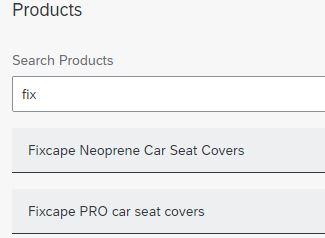
\includegraphics[width=0.5\textwidth]{Bilder/appgyver/4_1_Suchfilter_in_AppGyver.jpg}
 \caption{Suchfilter in AppGyver}
\end{figure}

In SAPUI5 ist die Integration eines Suchfilters durch das Hinzufügen von weiteren Controls und einem Filter auf dem AggregationBinding der Liste möglich. Das SearchField-Control verfügt bereits über das notwendige Verhalten und die zu konfigurierenden Eigeschaften und Events. Das Search-Event wird ausgelöst, wenn der Benutzer Werte in das Suchfeld eingegeben hat und dies per Button-Druck oder Drücken der Enter-Taste bestätigt. (Siehe Quelltext 4.1) 
\lstset{
  numbers=none, 
  basicstyle=\scriptsize,
  xleftmargin=.02\textwidth,
  backgroundcolor=\color{mygrey2},
}
\begin{lstlisting}[language=XML,  caption=Implementierung von Suchfilter in der \texttt{Main.view.xml}]
<List items="{path:'/Products'}" id="productsList">
	<headerToolbar>
		<OverflowToolbar width="100%">
			<SearchField width="200px" 
				placeholder="SearchProduct" 
				search="mySearchProduct" />
		</OverflowToolbar>
	</headerToolbar>
</List>
\end{lstlisting}

Das Search-Event wird im Controller in der Methode \textit{mySearchProduct} implementiert. Über das UI5Event-Object kann dort der Suchwert als Parameter abgerufen werden. Mittels manuellem Zugriff auf die Tabelle kann das ODataListBinding angesprochen und durch die Verwendung von Filtern auf den Suchwert gefiltert werden. Dem Coding ist zu entnehmen, dass wir nur auf die Title-Eigenschaft filtern. Direkt beim Setzen des Filters wird das ODataModel das Binding aktualisieren, die gefilterten Daten vom OData-Backend anfragen und die Liste an Produkten in der UI aktualisieren.
 
\begin{lstlisting}[emph={event, UI5Event, query, productsList, items, table, binding, filters},  caption=Implementation von Suchfilter in der \texttt{Main.controller.ts}]
public mySearchProduct(event:UI5Event){
const query = event.getParameter("query");
MessageBox.show(query);
const table = this.getView().byId("productsList");
const binding = table.getBinding("items") as ODataListBinding;
const filters = [];
if(query){
	filters.push(new Filter("title", FilterOperator.Contains, query))
}
binding.filter(filters);
}
\end{lstlisting}

\section{Integration von Paginierung}

Die Paginierung in Fiori Elements ist bereits als Standard-Funktionalität vorhanden. Per Default werden in einer Fiori-Elements-Anwendung 30 Listeinträge auf einer Seite angezeigt. Sind weitere Einträge vorhanden, werden erst beim Scrollen automatisch weitere 30 Listeinträge geladen, bis alle Datensätzen abgerufen werden. Die Standardeinstellungen können in Low-Code Kontext nicht geändert werden.

SAP AppGyver bietet für Listenansichten keine native Unterstützung einer Paginierung. Das Verhalten kann jedoch nachgebaut werden. Hierfür werden eine List-Component und zwei Buttons zur Steuerung der Paginierung benötigt. Zusätzlich sind zwei App-Variablen notwendig, eine zum Speichern der Seitennummer (pageNumber) und die andere zum Speichern der Gesamtzahl der Einträge (recordCount). Die Logik wird dann in einer Ablauffunktion (siehe Abbildung 4.2) implementiert. In Ablauffunktion „Get record collection“ werden zunächst die Daten von Backend geholt. Danach wird das Paging mit einem Custom Object definiert, in welchem die Page size (wie viele Einträge auf einer Seite angezeigt werden) und Page number  (aktuelle Seite) abgelegt werden. (siehe Abbildung 4.3).

\begin{figure}[htbp]
 \centering
 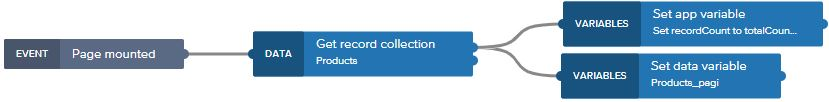
\includegraphics[width=1.0\textwidth]{Bilder/appgyver/4_2_Seitenlogic paginierung.jpg}
 \caption{Seitenlogik von Paginierung in AppGyver}
\end{figure}
 
\begin{figure}[htbp]
 \centering
 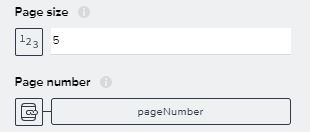
\includegraphics[width=0.5\textwidth]{Bilder/appgyver/4_3_Paging_definieren.jpg}
 \caption{Paging definieren in Ablauffunktion „Get record collection“}
\end{figure}

Damit die Paginierung funktioniert, müssen muss die Logik der Buttons noch hinzugefügt werden. Für beide Buttons gibt es eine eigene Ablauffunktion. Abbildung 4.4 zeigt die Logik der Buttons. Für PREV-Button wird den Wert der App-Variable „pageNumber“ mit folgender Formel ermittelt: 

\textit{\footnotesize SUBTRACT(appVars.pageNumber, 1)} 

Für NEXT-Button wird antstatt der SUBSTACT-Function die ADD-Function verwendet: 

\textit{\footnotesize ADD(appVars.pageNumber, 1)}

Damit der PREV-Button auf Seite 1 und der NEXT-Button auf der Letzen Seite ausgeblendet werden, muss die Sichtbarkeit der Buttons über das Visible-Flag gesteuert werden. Hier wird jeweils auf eine Formel verwiesen. Die Formel für PREV-Button lautet:  

\textit{\footnotesize NOT(IS\_EQUAL(appVars.pageNumber, 1))}

Die Formel für NEXT-Button sieht wie folgt aus:

\textit{\footnotesize MULTIPLY(appVars.pageNumber, 4) <= appVars.recordCount}

\begin{figure}[htbp]
 \centering
 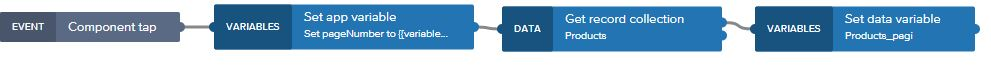
\includegraphics[width=1.0\textwidth]{Bilder/appgyver/4_4_Logik_PREV_und_NEXT.jpg}
 \caption{Logik für PREV- und NEXT-Button in AppGyver}
\end{figure}

Abbildung 4.5 zeigt die Benutzeroberfläche in der AppGyver-Anwendung, nachdem die Paginierung implementiert wurde.

\begin{figure}[htbp]
 \centering
 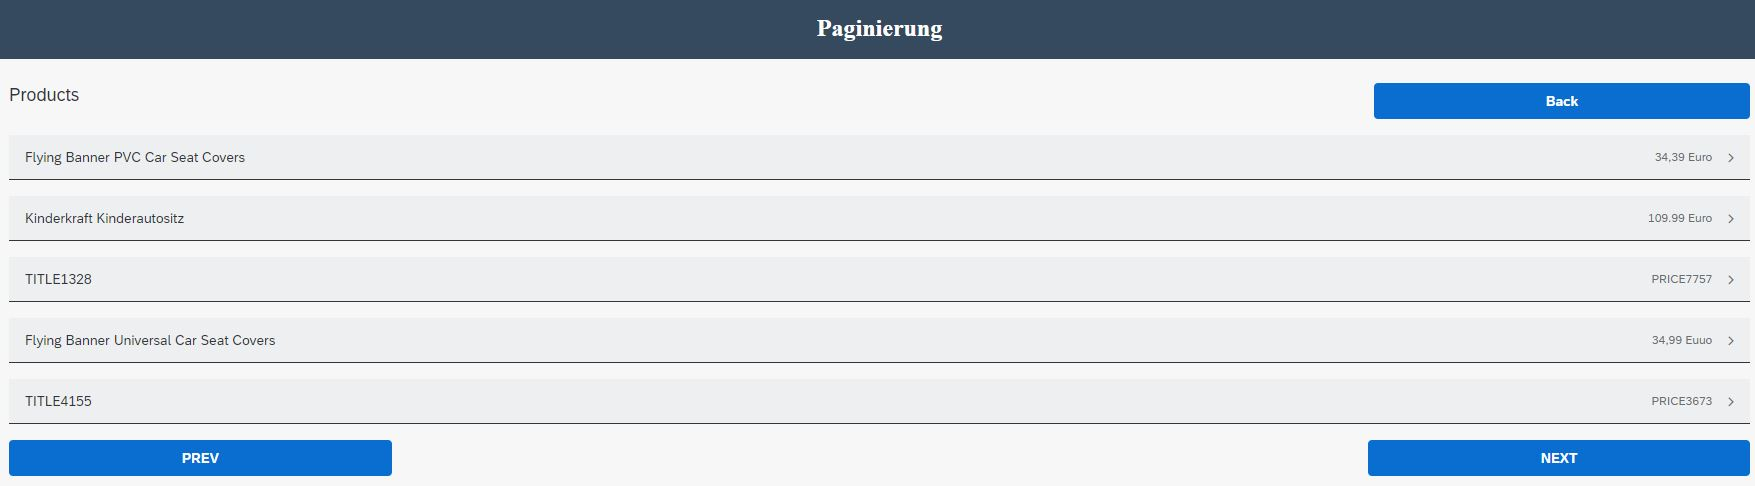
\includegraphics[width=1.0\textwidth]{Bilder/appgyver/4_5_AppGyver_pagnierung.jpg}
 \caption{Benuteroberfläche nach Paginierung in AppGyver }
\end{figure}

Die Integration der Paginierung in SAPUI5 ist sehr einfach, denn die entsprechenden List-Controls haben das Verhalten bereits implementiert. Setzt man die Eigenschaft \textit{growing} auf \textit{true}, dann wird das Nachladeverhalten bei Scrollen aktiviert. Eine weitere Property \textit{growingThreshold} kann hinzugefügt werden, um die Anzahl der Listeneinträge auf einer Seite zu bestimmen. Quelltext 4.3 zeigt nur mit 2 Zeile Code kann der Paginierung in SAPUI5 implementiert werden.
\begin{lstlisting}[language=XML,  caption=Implementation von Paginierung in der \texttt{Main.view.xml}]
<List growing="true" growingThreshold="8">
</List>
\end{lstlisting}

\section{Integration von Bild- und PDF-Datei}

Die Integration von Bild und PDF-Dateien in Fiori Elements ist im Low-Code Kontext nicht ohne weiteres möglich, da es in Fiori Elements derzeit noch keine Annotationen gibt, Datei-Formate auszuweisen. Grundsätzlich unterstützt das verwendete SAP Cloud Application Programming Model (CAP) die Bereitstellung von Mediendaten\cite{sapc:smd}, aber diese können nicht automatisiert in der UI dargestellt werden.

Auf der Seite von SAP CAP-Dokumentation kann man das Datenmodell wie folgt annotieren, um darauf hinzuweisen, dass die Entität Mediendaten enthält:

\begin{itemize}[noitemsep]
\item \textit{@Core.Media Type} gibt an, dass das Element Mediendaten enthält. 
\item \textit{@Core.IsMediaType} gibt an, dass das Element einen MIME-Typ enthält. MIME ist die Abkürzung für Multipurpose Internet Mail Extensions und bedeutet Internet Media Type\cite{mi:pag}.
\item \textit{@Core.IsURL@Core.MediaType} gibt an, dass das Element eine URL enthält, die auf die Mediendaten verweist.
\item \textit{@Core.ContentDisposition.Filename} gibt an, dass das Element als Anhang angezeigt werden soll, der heruntergeladen und lokal gespeichert wird.
\item \textit{@Core.ContentDisposition.Type} kann verwendet werden, um den Browser anzuweisen, das Element inline anzuzeigen.
\end{itemize}

Um die Medienressourcen zu lesen, sollte die GET-Anfrage in der Form \textit{/Entity/mediaProperty} verwendet werden. Um eine Medienressource zu erstellen, müssen wir zunächst eine Entität ohne Mediendaten erstellen, indem wir eine POST-Anfrage an die Entität stellen. Nach der Erstellung der Entität kann die Medien-Property mit der PUT-Methode eingefügt werden\cite{sapc:smd}. 

Die Integration von Bild-Dateien in AppGyver ist relativ einfach zu implementieren. Hierzu gibt es in AppGyver ein Standard-View-Component Image. Mit Drag and Drop kann diese Komponente zur Benutzeroberfläche hinzugefügt werden. 

Es gibt verschiedene Möglichkeiten, Bilder an die Benutzeroberfläche zu binden. (Abbildung 4.6) Mit „static image“ lässt sich ein lokales Bild auswählen und direkt hochladen. Wenn die Datei unter einer externen URL erreichbar ist, kann diese per "Formula" eingegeben werden. Weiterhin ist es möglich, auch Bilder aus Datenstrukturen auszulesen. Zudem gibt es im Marketplace verschiedene Ablauffunktionen, um die Kamera eines (mobilen) Endgeräts zu öffnen und ein Foto zu machen („Take photo“) oder ein Bild aus der Bibliothek des Geräts auszuwählen („Pick image from library“).

\begin{figure}[htbp]
 \centering
 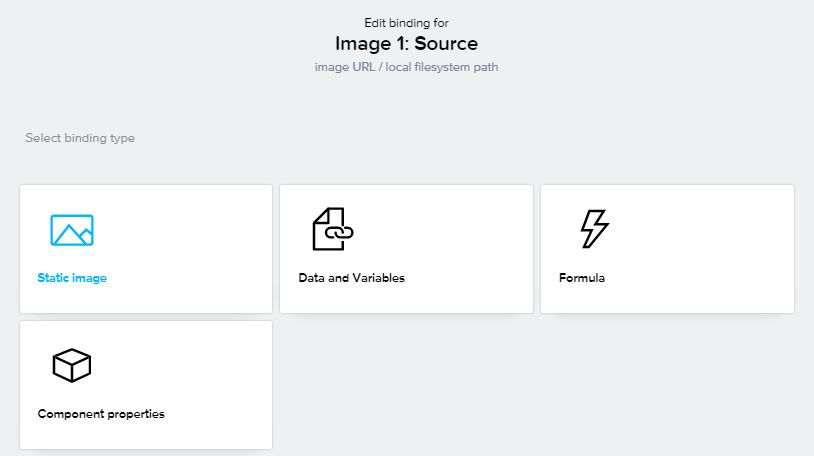
\includegraphics[width=0.7\textwidth]{Bilder/appgyver/4_6_Image_binding_in_AppGyver.jpg}
 \caption{Image Binding in AppGyver}
\end{figure}

Die Integration von PDF-Dateien in AppGyver erfordert ebenfalls nur einen geringen Implementierungsaufwand. Im Marketplace existiert eine Ablaufkomponente „Preview PDF“, welche an einen Button angehangen werden kann. In den Eigenschaften der Ablaukomponente kann dann dynamic oder statisch die URL der PDF-Datei angegeben werden. Abbildung 4.7 zeigt die Logik einen Flow mit der integrierten Ablaufkomponente. 

\begin{figure}[htbp]
 \centering
 
\includegraphics[width=0.7\textwidth]{Bilder/appgyver/4_7_Logik_Load-PDF-Button.jpg}
 \caption{Logik für Load-PDF-Button in AppGyver}
\end{figure}

Für die Integration von Bild- und PDF-Dateien in UI5 stehen Standard-Controls zur Verfügung, die mit geringem Konfigurationsaufwand einsetzbar sind. Für Bilder kann in SAPUI5 die Control „Image“ der sap.m-Library verwendet werden. Via „src“-Property kann ein relativer oder absoluter Pfad zur URL hinterlegt werden. Zudem kann man auch die Größe („width“-Eigenschaft) oder Höhe („height“-Eigenschaft) bestimmen. Mit der Standard Control „PDFViewer“ kann man PDF-Dateien integrieren. Hier gibt es eine „source“-Eigenschaft, die den Pfad zu der anzuzeigenden PDF-Datei enthält. Quelltext 4.4 zeigt die Implementierung von Bild- und PDF-Datei Integration in UI5 auf Basis einer XML-View.
\begin{lstlisting}[language=XML,  caption=Implementierung Bild- und PDF Datei Integration in SAPUI5]
<Image src="https://prod.pictures.autoscout24.net/listing-images/0693be87-aaad-4dc8-99c5-a69b3bd48b81_1934e390-16f2-4e47-b248-02e9cc9b746b.jpg"
           width="200px" height="150px"/>
<PDFViewer source="https://www.uni-muenster.de/imperia/md/content/zns/dokumente/beispielexpos___kowi_empirisch.pdf"/>
\end{lstlisting}

\section{Integration von Barcode-Scanner-Funktion}

Die native Integration einer Barcode-Scanner-Funktion in Fiori-Elements ist nicht vorgesehen. Über eine Extension könnte ein Button in der UI platziert werden, die eine solche Funktion bereitstellt. Die Logik dafür entspricht der SAPUI5-Implementierung (s. unten).

In AppGyver existiert eine Ablauffunktionskomponente „Scan QR/Barcode“, welche die direkte Integration einer Barcode-Scan-Funktion ermöglicht. Das triggern der Scan-Funktion kann über einen Button angestoßen werden. Abbildung 4.6 zeigt die Logik für einen Scan-Button. Die Scan QR/barcode Ablauffunktionskomponente kann dann mit dem Event „Component tap“ verbunden werden. Die Ablauffunktion hat mehrere Ausgänge: Es ist möglich, den Textinhalt des gescannten QR-Barcodes zu erhalten. Weiterhin kann man ebenfalls eventuell auftretende Fehler erhalten. Nachfolgende Abbildung zeigt die exemplarische Integration und Ausgabe von gefundenen Barcodes oder Fehlern in einem Dialog.

\begin{figure}[htbp]
 \centering
 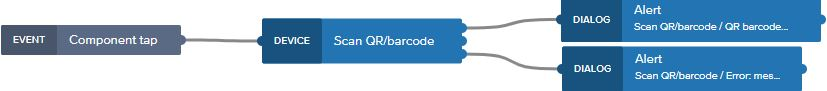
\includegraphics[width=1.0\textwidth]{Bilder/appgyver/4_8_logik_scan_barcode.jpg}
 \caption{Logik für Scan QR/Barcode-Button in AppGyver}
\end{figure}

Die AppGyver-Anwendung kann sowohl als Webanwendung, als auch als mobile Anwendung eingesetzt werden. Die Barcode-Scanner-Funktion wird von der AppGyver allerdings in einer Desktop-Webanwendung nicht unterstützt, sondern funktioniert nur auf mobilen Endgeräten.

In SAPUI5 existieren mehrere Barcode-Scanner-Controls.  Der Barcode Scanner Button (Namespace: sap.ndc) ist nur für die Nutzung auf mobilen Endgeräten vorgesehen (\textit{ndc} steht für \textit{native device capabilities}) und kann nur in Applikationen genutzt werden, die in der SAP Fiori Client-App geöffnet werden. Die neuere Komponente Barcode Scanner Dialog (Namespace: sap.ui.webc.fiori) kann dagegen auf allen Endgeräten im Browser eingesetzt werden.

Die Integration in eine Anwendung erfolgt durch Integration der jeweiligen Control in die View. In folgendem Beispiel wird ein BarcodeScannerButton integriert. Die Control stellt dann entsprechende Events bereit (\textit{scanSuccess} und \textit{scanFail}), die nach erfolgreicher oder fehlerhaftem Scan-Vorgang geworden werden. 
\begin{lstlisting}[language=XML,  caption=Implementierung Barcode-Scanner in View \texttt{Barcode.view.xml}]
<mvc:View controllerName="tff.Products.controller.Barcode" displayBlock="true" xmlns:ndc="sap.ndc" xmlns="sap.m" xmlns:mvc="sap.ui.core.mvc">
<VBox class="sapUiSmallMargin">
		<ndc:BarcodeScannerButton
			id="button"
			scanSuccess="onScanSuccess"
			scanFail="onScanError"
			dialogTitle="Barcode Scanner Button Sample"
		/>
		<HBox class="sapUiTinyMarginTop">
			<Label text="Scan Result:"/>
			<Text id="result" text="" class="sapUiTinyMarginBegin"/>
		</HBox>
	</VBox>
</mvc:View>
\end{lstlisting}

Im Controller kann die Callback-Funktion dann den Wert des Barcodes oder den Fehler aus den Event-Parametern auslesen. In folgendem Beispiel werden die Informationen auf dem Bildschirm in Form eines MessageToasts ausgegeben. 
\begin{lstlisting}[emph={event, cancelled, duration, text, Scan failed, Scan cancelled},  caption=Implementierung Barcode-Scanner in Controller \texttt{Barcode.control.ts}]
public onScanSuccess(oEvent) : void {
	if (oEvent.getParameter("cancelled")) {
		MessageToast.show("Scan cancelled", { duration:1000 });
	} else {
		if (oEvent.getParameter("text")) {
			oScanResultText.setText(oEvent.getParameter("text"));
		} else {
			oScanResultText.setText('');
		}
	}
}

public onScanError(oEvent) : void {
	MessageToast.show("Scan failed: " + oEvent, { duration:1000 });
}
\end{lstlisting}

\section{Nutzung nativer mobiler Funktionen}

Der Zugriff auf native mobile Funktionen, wie z.B. Sensor-Informationen des Smartphones, wird heute von modernen Browsern untersützt und ermöglicht die Nutzung in Applikationen.

SAP Fiori Elements-Apps greifen standardmäßig nicht auf native Funktionen zurück. Hier können über Extensions Funktionalitäten hinzugefügt werden, was jedoch einen Programmieraufwand mit sich bringt (s. SAPUI5 unten).

SAP AppGyver unterstützt den Zugriff auf Sensordaten durch die Bereitstellung von Flow-Funktionen, sowie spezisischen Sensor-Variablen. Diese können bei der Erstellung einer Anwendung berücksichtigt werden. Folgende Sensoren werden unterstützt:

\begin{itemize}[noitemsep]
\item Accelerometer 
\item Barometer
\item Kompass
\item Geolocation (GPS) 
\item Gyroscope
\item Magnetometer
\end{itemize}

SAPUI5 bietet im Namespace \textit{sap.ui.Device} grundlegende Informationen wie den Namen des Browsers oder der Plattform des Endgeräts, auf dem die Anwendung läuft. Tiefergreifende Funktionen zum Zugriff auf Sensordaten sind  jedoch nicht verfügbar. Hierfür lässt sich im Coding jedoch auf die APIs der Browser zugreifen und die entsprechenden Informationen in den UI5-Anwendungen nutzen.

\section{Möglichkeiten zum Deployment für unterschiedliche Endgeräte}

Standardmäßig können Fiori-Elements-Anwendungen und SAPUI5-Anwendungen nur als Webanwendung deployed werden. Es gibt dennoch unterschiedliche Möglichkeiten, eine Anwendung als App auf ein mobiles Endgerät zu bekommen. Die SAP bietet mit dem SAP BTP SDK für iOS eine native Implementierung von SAP Fiori an, die für diese Zwecke genutzt werden sollte. Quellcode oder Applikationslogik muss hier allerdings nativ in Apple Xcode und den iOS-Technologien implementiert werden. Daneben steht mit der SAP Fiori Client-App eine spezielle App zur Verfügung, mit der SAPUI5-Anwendungen auf einem mobilen Endgerät geöffnet werden können. Die Applikation wird allerdings weiter als Webapplikation deployed.

In AppGyver gibt es mehrere Möglichkeiten, die erstellte Anwendung zu deployen. Hierfür steht der SAP AppGyver Build Service zur Verfügung, der die Anwendungen Verpacken und auch direkt Verteilen kann. Die Deployment-Optionen sind folgende:

\begin{itemize}[noitemsep]
\item \textbf{Android Builds} 

Eine Anwendung kann via Android SDK in eine native Android-App verpackt werden. Nach dem Bauen der Anwendung, kann diese mit einem USB-Kabel auf dem Gerät installiert werden oder als Direkt-Download-Link weitergegeben werden.  Es ist ebenfalls möglich, die App über den Google Play Store oder andere Android-App-Management-Lösungen zu veröffentlichen. Die Dateigröße von Android kann sehr groß sein, da die Binärdatei optimierte Unterstützung für mehrere verschiedene Prozessoren enthält\cite{app:bu}. 
\item \textbf{iOS Builds} 

Das Bauen als native iOS-App erfordert zunächst die Mitgliedschaft im Apple Developer Programm. Über das Apple Developer Portal können dann die benötigten Anlagen generiert, konfiguriert und die App gebaut werden. Nach der Generierung lässt sich die App an die Mitglieder der Apple Developer-Organisation verteilen. Ebenso ist es möglich, die App zur Review an Apple senden. Nachdem die App angenommen wurde, ist sie im öffentlichen App Store verfügbar\cite{app:ios}. 
\item \textbf{Web Builds} 

Bei der Veröffentlichung als Webanwendung mit dem Build Service, wird die Anwendung in der AppGyver Cloud unter der von uns definierten und konfigurierten Subdomain bereitgestellt.
\end{itemize}

\section{Freie Gestaltungsmöglichkeit}

Fiori-Elements basieren auf den SAP Fiori Design Guidelines und den fest definierten Floorplans (siehe Kapitel 2.6.1). Zwar sind durch die Extension-Points und dem Hinzufügen eigener Controls geringe Abweichungen im Layout möglich, die Gestaltungsmöglichkeiten bleiben jedoch sehr beschränkt. Durch die Auswahl eines eigenen SAPUI5-Themes oder dem Überschreiben von CSS-Anweisungen könnte das Aussehen weiterhin beeinfluss werden. Die Grundidee hinter Fiori Elements, leicht zu erstellende sowie gleich aussehende und funktionierende Standard-Apps, steht jedoch generell im Widerspruch zur Idee der freien Gestaltungsmöglichkeiten.

In AppGyver ist es möglich, die Anwendungen nach dem Designvorlieben eines Nutzers zu entwickeln. Der Themen-Editor in Composer Pro ermöglicht die Auswahl, sowie die Anpassung von Themen für die Anwendungen. Ein Theme bezeichnet dabei das grundlegende visuelle Erscheinungsbild einer Anwendung und definiert Schriftgröße und -art, Farben der UI-Elemente sowie Hintergrundbilder\cite{hel:the}. Themes besitzen zudem Inhaltspaletten und semantischen Farben, mit denen eine Anwendung gezielt Formattierungen bereitstellen kann\cite{appg:the}. Als grundlegende Themes stehen in AppGyver zwei Themes bereit: 

\begin{itemize}[noitemsep]
\item Das universelle Theme ist ein modernes Allround-Theme, das sich einfach als Basis für ein individuale Theme adaptieren lässt.
\item Das SAP-Fiori-Theme hilft bei der Implementierung des SAP Fiori Designsystems in AppGyver-Anwendungen\cite{har:new}.
\end{itemize}

Im AppGyver Composer Pro haben alle View-Components Style-Klassen und Layout-Parameter. Die Style-Klassen definieren, wie eine Komponente in der UI aussieht, einschließlich Schriftart, Farben, Rahmen usw. Damit lassen sich allgemeine Werte aus den Themes überschreiben. Der Layout-Parameter bestimmt, wie eine bestimmte Komponenten auf der aktuellen Seite angeordnet wird (Abstand, Breite und Höhe und Position). Die Style und Layout können je nach Präferenz des Benutzers angepasst werden. Abbildung 4.9 zeigt 3 verschiedene Gestaltungen von AppGyver Anwendungen.

\begin{figure}[htbp]
 \centering
 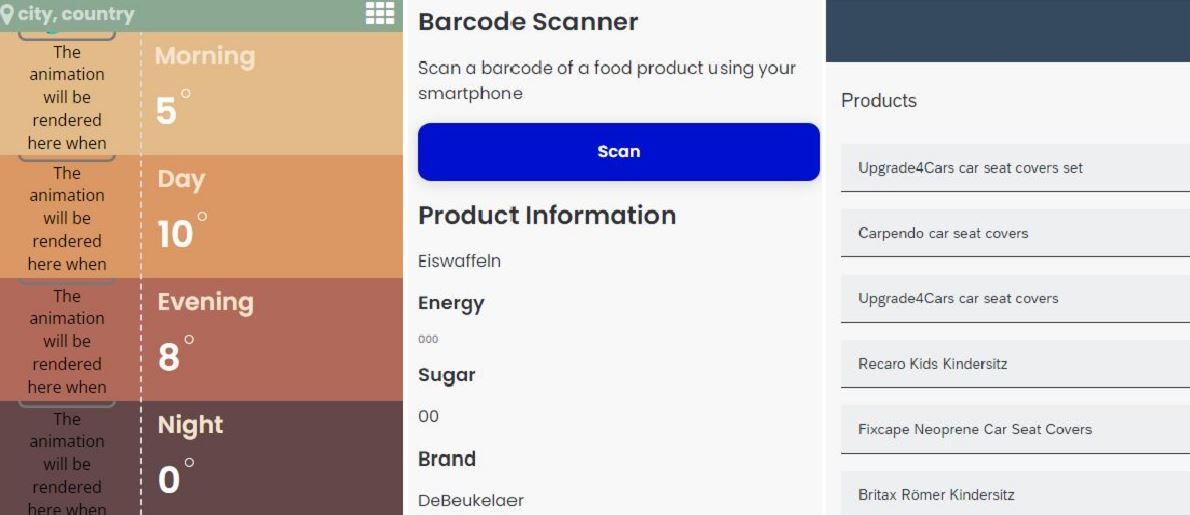
\includegraphics[width=1.0\textwidth]{Bilder/appgyver/4_9_1_gestaltung.jpg}
 \caption[1]{Gestaltung von Weather-App, Barcode-Scanner-App\footnotemark und Product-List-App\footnotemark }
\end{figure}
\addtocounter{footnote}{-1}
\stepcounter{footnote}\footnotetext{Weather-App wurde nach dem Youtube AppGyver-Tutorial von Iyad Helwani erstellt. URL: https://www.youtube.com/watch?v=ktb8so0mKmI\&t=1819s} 
\stepcounter{footnote}\footnotetext{Barcode-Scanner-App wurde nach SAP Tutorial von Daniel Wroblewski erstellt. URL: https://developers.sap.com/tutorials/appgyver-create-application.html}

SAPUI5 orientiert sich zunächst ebenfalls an den SAP Fiori Guidelines. Anders als in Fiori Elements ist man jedoch beim Aufbau einer Anwendung in „freestyle“-Apps komplett frei. Auch das Design lässt sich anpassen, hier gibt es zwei Möglichkeiten:

\begin{itemize}[noitemsep]
\item \textbf{Gestaltung einzelner UI-Elemente mit CSS } 

Einzelne Controls in SAPUI5 können durch die Vergabe von speziellen CSS-Klassen mit eigenen Style-Definition umgesetzt werden\cite[S.261]{sapui5}. Zudem ist es möglich, gezielt existierende Styles zu überschreiben.
\item \textbf{Erstellung eigenständiger Themes mit Theme Designer} 

SAPUI5 unterstützt ebenfalls Themes. Ein benutzerdefiniertes Theme kann mit dem UI-Theme-Designer erstellt werden. In einem Theme werden verschiedene Parameter (Schriften, Farben, etc.), Bilder und andere Ressourcen konfiguriert, die dann einen Einfluss auf alle Controls einer Anwendung haben\cite{saph:bas}. 
\end{itemize}






